\chapter{BACKGROUND}
\label{background}
%Some mathematical techniques which are used to solve the problems in thesis are introduced in this chapter.
%Neel06analysisand

In contrary to game theory where players agree on an equilibrium via autonomous behaviours, optimization problem, which attempts to optimize the welfare of either one equipment or whole network, is usually conducted on a single decision maker.
In the following, we introduce some basics of game theory and optimization.





 

%\todo[inline]{expand: Introduction of game theory...}
\section{Introduction of Game}
%Game theory is established by Nash in xxxx, and is applied in network communication since xxx
In this section, we give a brief introduction of game theory and congestion game which is applied to solve problems in the dissertation.
The notations used in this thesis comply with~\cite{agt_book}.


%\subsubsection*{Strategic Game}

A game of normal form can be represented as a tuple $\Gamma = (\mathcal{N}, (\Sigma_i)_{i \in \mathcal{N}}, (u_i)_{i\in \mathcal{N}})$, where 
\begin{itemize}
\item $\mathcal{N}$ is a finite set of players.
\item $\Sigma_i$ is player $i$' set of strategies.
Player $i$ selects one strategy $\sigma_i\in \Sigma_i$ at one time to play the game.
\item $\Sigma = \Sigma_1\times\cdots\times \Sigma_n$ is the set of states, which denotes all the possible ways that players may pick strategies.

\item $\sigma=(\sigma_i,\cdots,\sigma_n)$ is one strategy, which represents an instance of all players' strategy choices.
$\sigma$ is also called one strategy profile, and there is $\sigma\in \Sigma$.

\item One vector of strategies of player $i$' opponents is expressed as $\sigma_{-i}$, and the corresponding strategy profile is denoted as $\sigma=\{\sigma_i, \sigma_{-i}\}$.
$u_i(\sigma) = u_i(\sigma_i, \sigma_{-i})$ is the player $i$' outcome in strategy profile $\sigma$.

\item $u_i: \Sigma\rightarrow \mathbb{R} $ is the utility function of player $i$.
%$\sum=\sqcap_{i\in \mathcal{N}}\sum_i$ is the set of states of the game, which denotes all the possible ways that players may pick strategies.
$\Sigma_{-i}=\prod_{j\in \mathcal{N}\setminus \{i\}}\Sigma_j$ is the set of states of all the other players except for player $i$.
As to each player $i$, its utility is decided by its choice on strategy $\sigma_i\in \Sigma_i$, and is also dependant on the choices of other players $\sigma_{-i}\in \Sigma_{-i}$.
Utility can also be denoted as $u_i(\sigma)$ or $u_i(\sigma_i,\sigma_{-i})$ to stress that the utility is made based on all players' strategies.


Utility function is very important to specify a game, as it gives players preferences on the outcomes with respect to all strategy vectors $\Sigma$.
The value of the utility can be regarded as payoffs or costs depending on concrete scenarios.
Actually, one player maximizes its utility is equivalent to that the player minimizes its cost, note that cost is the reversed utility.
%The sum of costs and payoffs are zero, and they can be used interchangeably.
\end{itemize}




When we want to use game theory to analyse a problem in CRN, it is critical to formulate appropriate components of the problem into corresponding elements of a game.
The commonly used formulation is summarized in Table~\ref{game_crn_component}.

\begin{table}
\centering
\begin{tabular}{|c|C{7cm}|}
\hline 
Elements of a game & Components of one CRN \\ 
\hline 
Player $\mathcal{N}$ & secondary users \\ 
\hline 
Strategies for player $i$, $\mathcal{S}_i$  & working channels, transmission power, modulation, etc. \\ 
\hline 
Utility of player $i$, $u_i$ & performance in respect of SINR, throughput, etc. \\ 
\hline 
\end{tabular} 
\caption{Components of problems in CRN and corresponding elements in game}
\label{game_crn_component}
\end{table}




\subsection{Basic Solution Concepts}
In this section, we will introduce some basic solution concepts, some of them are used in this thesis.
\subsubsection*{Dominant Strategy Equilibrium}
In some games, each player has a unique best strategy, which is independent of the strategies chosen by the other players, then we say a game of this kind has a dominant strategy solution.
The mathematical expression is, a strategy vector $s\in \mathcal{S}$ is a dominant strategy, if for each player $i$ and each alternate strategy $s'\in \mathcal{S}$, there is, 
 \[ u_i(s_i, s_{-i}') > u_i(s_i', s_{-i}')\]
$s$ is also called strong dominant strategy, and when the $>$ can be written as $\geq$, $s$ is called weak dominate strategy.
Note that a dominant strategy solution may not give an optimal payoff to any of the players.
This is the case in \textit{prisoner's dilemma}, which is one of the most well known and well studied games.
To confess is the dominant solution for both prisoners, which brings them longer time behind bars than that when both of them keep silent\footnote{Prisoner's dilemma can be found in almost all the game theory textbooks, thus omitted in this thesis.}.
Only a few games have dominant strategy equilibrium, and mechanism design~\cite{Design_Mechanisms_1973} is developed to design games which have dominate strategy equilibrium, and these dominate strategies lead to desirable outcome.



\subsubsection*{Nash Equilibrium}
A desirable solution of games is the one that players choose strategy in accordance with their incentives, minimizing their own cost or maximizing their own payoff/utility.
Nash equilibrium successfully captures this property, and is the most discussed and pursued solution concept in game theory.

A strategy vector $s\in S$ is a \textit{Nash equilibrium} if for any player $i$ and each alternate strategy $\sigma_i'$, there is
 \[ u_i(\sigma_i, \sigma_{-i}) \geq u_i(\sigma_i', \sigma_{-i})\]
This means for any player in NE state, no unilateral deviation from its current strategy is more profitable.
This also implies that, NE is self enforcing that once players agree on this solution, it is the best interest for every player to stick to its current strategy.

A dominant strategy equilibrium is a Nash equilibrium, but a NE is not necessarily a dominant strategy.
There may be multiple NEs in one game, and NE may not be optimal for players. 
In prisoner dilemma, the dominating strategy is NE but is obviously not the optimal.


Being not unique and possibly sub-optimal, NE is still applied in extremely diverse applications due to the reasons discussed in the beginning of this section.
Thus, when pursuing NE as solution, people should answer the question that, what is the gap between NE and global optimal?
This can be partially answered by \textit{price of anarchy (\gls{PoA})}, the ratio between the worst-case Nash equilibrium to the optimality is used to denote the quality of the solution.

Nash equilibrium is an appealing concept, but it doesn't tell how to reach such a state.
Hence, it is important to find an efficient algorithm to reach the equilibrium.
The notion of \textit{NP-completeness} is not an appropriate concept of complexity for \textit{finding a Nash equilibrium} problem as NE always exists, nevertheless, theoretical scientists tell \textit{finding a Nash equilibrium} problem is a combinatorial problem and is often very difficult (Chapter 2, \cite{agt_book}).
Having said that, in some games, with the special strategy space structure, or players' special behaviours, efficient algorithms to reach NE exist.





%Nash equilibrium is a conceptual tool and a prediction about the rational strategic behaviour by agents in situations of conflict, hence, it carries great importance to know how much computational effort needed to compute NE.



%\subsubsection*{Pareto Optimality}
%%There exists other equilibrium conceptions. \ie Pareto Equilibrium . 
%An strategy profile $\bar{s}$ is \textit{Pareto optimality} (\gls{PO}), if there does not exist profile $s$ with $u_i(s)\geq u_i(\bar{s})$ for each $i\in N$, and meanwhile $u_i(s)> u_i(\bar{s})$ for at least one $i\in N$.
%PO is the necessary condition of the global optimality and accordingly is more favoured, but its application in communication system is much less than NE because it is not easy to obtain, and the lack of stability.


\subsubsection*{Pure NE and Mixed NE}
In the aforementioned games, players deterministically choose one strategy from theirs strategy sets, then play their chosen strategies and don't involve randomized strategies, then the achieved NE is called pure NE. 
When players play a game with certain randomization on strategies, and aim to maximize their expected payoff, we call the resulted NE as mixed NE.
As to mixed NE, the action of a player is to choose certain strategies according to a probability distribution.
Games with finite number of players and strategy set are guaranteed to have NE, whereas, games with an infinite number of players, or games with a finite number of players but they can access to an infinite strategy set may not have NE~\cite{agt_book}.

In this thesis, we only consider pure NE, as players deterministically play a certain strategy, and the corresponding network components stick to certain operation instead to switch among several different operations based on a vector of probabilities.
Other solutions include correlated equilibrium, which also involves probability distribution over strategy vectors.


%Unlucky, the computation of NE is usually a combinatorial optimization problem (chapter 2)~\cite{}.
% but in some special cases, 

%\subsubsection*{Different Games in Nutshell}


\subsubsection*{Individual Optimization and Game}
As to a player in a game, given the strategies of other players $\sigma_{-i}$, its utility $u_i$ is a function of its own strategy $\sigma_i$, then the maximization of its payoff or minimization of its cost becomes one optimization problem.
Thus, one game comprises $n$ such optimization problems in total.
%Whereas as to a general game, the payoff or cost of each player depends on both $s_i$ and $s_{-i}$, both its own strategy and the strategies chosen by all other players.





\section{Congestion Game}
\label{congsetion_game}

%\subsubsection*{Congestion Game}

%Congestion game is a special type of potential game, which has extra conditions, but also yield favourable characteristics.

%In congestion game, player pays for the resources it occupies.
%Particularly, the payment for one resource is monotonically increasing with the \textit{number} of players occupying that resource, and each player tries to minimize its payment~\footnote{Another way to describe congestion game: player gets benefit by using a certain resource, the benefit is monotonically decreasing with the number of players on that resource, each player tries to maximize its welfare}. 

Congestion game is an attractive game model which describes the problem where participants compete for limited resources in a non-cooperative manner, it has good property that Nash equilibrium can be achieved after finite steps of best response dynamic.
Congestion game has been used to model certain problems in internet-centric applications or cloud computing, where self-interested clients compete for the centralized resources and meanwhile interact with each other.
For example, server selection is involved in distributed computing platforms~\cite{Cloud_Computing_2010}, or users downloading files from cloud, etc.
In the following we will introduce an \textit{server matching}~\cite{kothari:congestion_serverMatching} problem to illustrate congestion game's application in communication systems.

In accordance with~\cite{Voecking06congestiongames}, congestion game is a game where players simultaneously allocate sets of resources to minimize their costs, and the cost of a resource is a function of congestion, which is the number of players choosing the resource.
Congestion games can be formulated from many problems in realistic world, \eg minimisation of commuting time on the road for commuters, minimization of energy consumption in mobile cloud computing system~\cite{game_cloudcomputing_energy12}.


Now we give the formal definition of a congestion game.
A congestion game~\cite{Rosenthal}\cite{Voecking06congestiongames} can be expressed by a tuple $\lambda=(\mathcal{N},\mathcal{R},(\Sigma_i)_{i \in \mathcal{N}},(g_r)_{r\in \mathcal{R}})$, where
\begin{itemize}
\item $\mathcal{N}=\left\{1,\ldots,N\right\}$ denotes the set of players (each each is labelled with a unique index number)
\item $\mathcal{R}=\left\{1,\ldots,m\right\}$ the set of resources
\item $\Sigma_i$ is the set of resources for player to use.
\item $\Sigma_{i\in\mathcal{N}} \subseteq 2^{\mathcal{R}}$ is the strategy space of player $i$. 
Under strategy profile $\sigma=(\sigma_1,\sigma_2,\cdots \sigma_N)$, player $i$ chooses strategy $\sigma_i\in \Sigma_i$, and the total number of users using resource $r$ is $n_r(\sigma)=|\{i\mid r\in \sigma_i\}|$. 
\item The cost $g_r: \mathbb{N}\rightarrow \mathbb{Z}$ is a function of the number of users for resource $r$, $g_r^i=\sum_{r\in \sigma_i} g_r(n_r(\sigma))$. 
\end{itemize}
In our paper, $g_r^i$ is referred as \textit{congestion} of a game.

We first give a definition of improvement.
\begin{mydef}
An improvement path is a path $(\sigma^0, \sigma^1, \cdots)$ in which $u_i(\sigma^k) < u_i(\sigma^{k+1}) $, where $\sigma^k$ and $\sigma^{k+1}$ differ in the player $i$'s coordination, \ie only $i$'s strategy changes in the strategy $\sigma={\sigma_1, \sigma_2, \cdots, \sigma_{|\mathcal{N}|}}$.
\end{mydef}
The best response path contains only states for best response improvement steps.


\begin{theorem}
\label{background:finiteImprovement}
For every congestion game, every sequence of improvement steps is finite.~\cite{Rosenthal}
\end{theorem}

This theorem immediately implies the following corollary,
\begin{corollary}
\label{background:corollary}
%\emph{Every congestion game has at least one pure Nash equilibrium.}
Every congestion game has at least one pure Nash equilibrium.~\cite{Rosenthal}
\end{corollary}

To prove this, let us first have a look at one similar game, potential game.
Potential game~\cite{Mondere_potential_game:1996} has already been applied in wireless network and CRN to help solve different problems~\cite{CApotentialLearning_05dyspan, caps_potential2012, self-coexistenceWRAN2010infocom, pimrc_2012}.
Potential game has two desiring properties, the existence of pure NE, and every improvement path is finite, which makes it a suitable model to design distributed algorithms.


\subsubsection*{Potential Game}

A potential game is a tuple $\lambda=(\mathcal{N},(\Sigma_i)_{i \in \mathcal{N}},(u_i)_{i\in \mathcal{N}})$, which satisfies the following, if there exists a function $\phi: \Sigma\rightarrow \mathbb{R}$, such that for every $i\in \mathcal{N}$, for every $\sigma_{-i}\in \Sigma_{-i}$, and every $\sigma_i, \sigma_i'\in \Sigma$:

\begin{equation}
\label{2:1}
\begin{split}
u_i(\sigma_i, \sigma_{-i})-u_i(\sigma_i', \sigma_{-i}) >= \phi_i(\sigma_i, \sigma_{-i})-\phi_i(\sigma_i', \sigma_{-i})
\end{split}
\end{equation}
If equality holds, this game is called an exact potential game, when it doesn't, the game is called an ordinal potential game.
It is easy to see that the design of potential function $\phi$ is the key point to form a potential game. 
The incentive of any player to change its strategy can be expressed using the potential function, in other words, potential game tracks the changes in the payoff/cost with some player deviates.


Potential game has two important theorems,
\begin{itemize}
\item Every finite ordinal potential game has at least one pure strategy Nash equilibrium.
\item In every finite ordinal potential game, every improvement path is finite.

\end{itemize}

%Based on potential game model, Rosenthal~\cite{Rosenthal} built a potential function,
\subsection{Convergence Time Towards Nash Equilibrium}
As to the Theorem~\ref{background:finiteImprovement} which implies the that, for every congestion game, every best response ends in finite steps, we introduce the sketch of the proof of this proposition, as the proof also reveals the number of steps needed to reach a Nash Equilibrium.
% ~\cite{Voecking06congestiongames} 
We first introduce Rosenthal's potential function $\phi(s):\Sigma\rightarrow \mathbb{Z}$, where $\sigma$ is the strategy profile of all the players, let $\sigma = \sigma_1, \sigma_2,\cdots, \sigma_N$:
\begin{equation}
\label{2:Rosenthal_potential}
\begin{split}
\phi(\sigma) 
& =\sum\limits^{}_{r\in \mathcal{R}} \sum\limits^{n_r(\sigma)}_{i=1} g_r(i)\\
& =\sum\limits_{i\in \mathcal{N}} \sum\limits^{}_{r\in s_i} g_r(n_r^i(\sigma))\\
\end{split}
\end{equation}
$n_r^i(\sigma)$ is the number of players using resource $r$, whose indices are smaller than or equal to $i$, \ie from $\{1,\cdots,i\}$. 
In the part after the second equality sign, $\sum\limits^{}_{r\in \sigma_i} g_r(n_r^i(\sigma))$ is a virtual value or cost that player $i$ have when assuming the resource $r$ is not used by players whose indices are greater than $i$.
%Note that the potential is \textit{not} the sum of congestions experienced by every user. 

The intuitive interpretation of the virtual cost is, according to~\cite{Voecking06congestiongames}, the cost of each player for choosing the strategy when it is inserted into the game.
Let us assume player $N$ is the last player to be inserted into the game, then $\sum\limits^{}_{r\in s_N} g_r(n_r^N(\sigma))$ equals to the real cost that player $n$ takes.
When player $N$ can decrease its cost by switching to another strategy by an unilateral move, then $\sum\limits^{}_{r\in \sigma_N} g_r(n_r^N(\sigma))$ and its potential decrease by the same amount.
As the potential can be calculated by inserting the players with any sequence, each player will have the same property with play $N$, as we just discussed.

In summery, the change of the potential caused by one player's unilateral move from $\sigma_i$ to $\sigma_i'$ is equivalent to the change of gain (or loss) of that player.
\begin{equation}
\label{5}
\varDelta \phi(\sigma_i \rightarrow \sigma_i') = g^i(\sigma',\sigma_{-i}) - g^i(\sigma,\sigma_{-i})
\end{equation}
$\sigma_{-i}$ is the strategy profile for all players except for $i$.
Thus the potential decreases with the update of players monotonically during the convergence process.
Most importantly, as the potential of a congestion game is bounded, and every best response move made by a player decreases it at least by 1, the length of any sequence of improvement steps is also finite.
Then the Theorem~\ref{background:finiteImprovement} is proved.



The existence of Nash equilibria gives a natural solution concept for congestion games.
Comparing with potential game, congestion game is much easier to connect with the problems in networks or CRN.
As long as we can decide the payoff (or cost) happened upon a certain resource, \ie spectrum bands, time slots, transmission power is monotonic increasing (or decreasing), we can formulate the problem into one congestion game, and we can make use of the property of congestion game to implement best response to achieve Nash equilibrium.


%As every congestion game is a potential game, and the total potential is finite, thus the number of improvements is upper-bounded by $2\cdot\sum\limits^{}_{r\in \mathcal{R}} \sum\limits^{n_r(\sigma)}_{i=1} g_r(i)$ \cite{Voecking06congestiongames}.

%\section{Application of congestion game in the design of decentralised algorithm}
%\todo[inline]{expand: the application of potential game in CRN}
\subsection{Singleton Congestion Game}
We introduce a special type of congestion game~\cite{aaai_IeongMNSS05}, which implies polynomial number of best response steps towards convergence.


\begin{mydef}
\label{background:singleton}
A congestion game is called singleton if, for every $i\in \mathcal{N}$ and every $\mathcal{R}\in \Sigma_i$, it holds that $|\mathcal{R}|=1$.
\end{mydef}
In words, each player allocates one single resource from its strategy set.
Although this constraint on the players strategies is very restrictive, there are still $m^n$ different strategy profiles.

\begin{theorem}
\label{background:polynomialConvergence}
In singleton congestion games, all improvement sequences have length $\mathcal{O}(n^2m)$~\cite{aaai_IeongMNSS05}
\end{theorem}

The sketch of the proof is as follows.
The upper bound on the number of convergence steps is shown in Formula~\ref{2:Rosenthal_potential}.
Now we need to approximate this expression.
Replace original delays by smaller integer values without changing the preferences of the player, then calculate an upper bound on the maximum potential with respect to the new delays.
For example, if the delay on a certain resource is 15, 50, 100 with respect to 1, 2 and 3 players using that resource, then we manipulate the delays as 1, 2, 3.
When the number of resource is $m$ and number of players is $n$, the largest new delay is $mn$.
Then the Rosenthal's potential in Formula ~\ref{2:Rosenthal_potential} has the following relationships with an upper bound.
\begin{equation}
\label{2:Rosenthal_potential_newdelay}
\begin{split}
\phi(\sigma) 
& =\sum\limits^{}_{r\in \mathcal{R}} \sum\limits^{n_r(\sigma)}_{i=1} g_r(i)\\
& =\sum\limits^{}_{r\in \mathcal{R}} \sum\limits^{n_r(\sigma)}_{i=1} nm\\
& \leq n^2m
\end{split}
\end{equation}
Therefore, the length of improvement sequences is upper-bounded by $n^2m$.
The proof in details can be found in ~\cite{aaai_IeongMNSS05, LectureA}


\subsubsection*{Example: Server Matching}
In order to show how is problem in networks formulated into a game, and from which an effective algorithm is proposed, we introduce a small example with the application of singleton congestion game.

Let us consider a number of self-interested clients and servers as shown in Figure~\ref{server_sharing}.
Each client is allowed to access one server.
The latency of one server is a monotonic increasing function of the \textit{number of clients} attached to it.
When clients try to choose one server which has the shortest latency, a congestion game is formed.
\begin{figure}[h!]
  \centering
  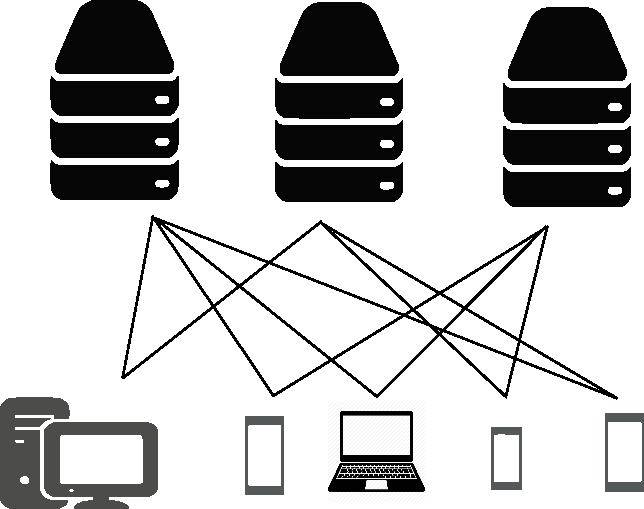
\includegraphics[width=0.6\linewidth]{server_sharing.pdf}
  \caption{An example server matching, one server is possible strategy of the client at the other end of the connecting line}
\label{server_sharing}
\end{figure}

Following the description in Section~\ref{congsetion_game}, we write the game for this problem, 
\begin{itemize}
\item The clients constitute the players in the game $\mathcal{N}$, and the collection of servers $\mathcal{M}$ is the strategy space for every player.
\item The cost of players in the game is equivalent to the latency for the clients .
If we denote the delay happens on the server as $d(n)$, where $n$ is the number of clients using the server, then the delay (cost) for a client (player) $i$ is $d(n_r(\sigma))$, where $n_r(\sigma)$ and $r\in \sigma_i$ is the number of clients using the server $r$.
\item As each user is allowed to use on server, this is a singleton congestion game according to Definition~\ref{background:singleton}.
\end{itemize}

Then, according to Theorem~\ref{background:finiteImprovement} and~\ref{background:polynomialConvergence}, after maximal $nm$ times best responses, the system reaches Nash equilibrium.
%More formally, this corresponding congestion game is composed of players (the self-interested clients) and resources (servers), where players are allowed to choose one certain resources to use. 
%There is cost (latency) generated on a resource for the players who use that resource, and the cost is monotonic increasing with the number of players using it. 
%As congestion game permits convergence when every players in turn adopt the strategy which leads to a better utility.



%Thus in server matching problem, when clients in turn choose a permissible server with a smaller predicted latency, then after finite number of steps, no client has motivation to switch any more, and we reach a NE.

%If every player greedily searches the allowed resources to decrease its cost, the dynamics will cease in Nash equilibrium, where no player has motivation to adopt a new set of resources unilaterally. 




\subsection{Variants of Congestion Game}
In the congestion game we have introduced in Section ~\ref{congsetion_game}, the cost caused on one resource is function of the number of players using that resource.
In some variants of congestion game, the cost is decided by some other factors.
In \textit{player specific congestion game}, different players may have different delay functions.
As to \textit{weighted congestion game}, different players may have different impacts on the delays of the resources they allocate, in other words, there is a weight for every player, and the congestion on a resource is the total weight of all players using that resource.

As to neither player specific congestion game nor weighted congestion game, the finite converge does not hold anymore.
But there exits NE for both of Player specific congestion game and weighted congestion game when they are singleton congestion game~\cite{Milchtaich1996111, FKKMS02}.
When these variant of congestion game are not singleton ones, \cite{Ackermann06purenash} points that NE exists when the strategy space of players are matroid.








\section{Optimization}

As discussed in Section~\ref{operation_model}, the available radio resources such as spectrum and transmission power are scarce, Meanwhile, new services raise new requirements for these resources.
Resource allocation and its optimization are needed to accommodate the needs.
Various optimization problems are formulated to improve radio resource usage in CRN~\cite{cacao_ca_2011, fuzzy_decision_09, resourceAllocation_imperfectSensing_2012}.
Optimization can be conducted from either a global view or from individual perspectives.

Many wireless resource allocation problems are formulated as constrained optimization problems.
Table~\ref{opt_table} shows the commonly used parameters, objectives and constraints of some optimization problems in wireless communication.
Part of the contents in Table~\ref{opt_table} refers \cite{Han:2008:RAW:1457343}.

\begin{table}
\begin{tabular}{|L{2.1cm}|C{3.8cm} | C{3.5cm} | C{3.7cm}|}
\hline 
 & Parametres & Optimization goals & Constraints \\ 
\hline 
Application layer & source-coding rate, buffer priority, packet arrival rate & minimal delay & base layer transmission, strict delay requirement \\ 
\hline 
Network layer & routing path & end to end delay/throughput & maximal hops, security concerns \\ 
\hline 
MAC layer & transmission frequency, transmission priorities & maximal overall throughput, minimal buffer overflow probability & contentions, time/frequency slot \\ 
\hline
Physical layer & transmission power, modulation, channel coding rate & minimal over power consumption, maximal throughput, minimal BER & maximal transmission power, caused interference on licensed users, available channel coding rate \\ 
\hline
\end{tabular} 
\caption{Optimization problem of cognitive radio networks}
\label{opt_table} 
\end{table}

The solutions to optimization problems can be categorized by their properties, \ie convex, linear, integer, or non-convex non-linear, etc.
In this thesis, we make use of different solvers, \ie Lindo, Gurobi, to solve the formulated optimization problems in different categories.


%Optimization outputs the results with the global information.
%Optimization is implemented on one entity, thus it is naturally suitable in centralized scheme.
